
\section{Preprocessing and Validation}

\begin{breakbox}
\boxtitle{Data Mining Process Steps}

\begin{itemize}
	\item \textbf{Data Integration}: gather data from multiple sources
	\item \textbf{Data Cleansing}: correct or remove noisy and inconsistent data
	\item \textbf{Data Selection}: source just the relevant data
	\item \textbf{Data Transformation}: reformat and prepare data according to algorithm requirements
	\item \textbf{Application of Algorithms}: detect patterns
	\item \textbf{Validation}: measure pattern quality and identify the most significant ones
	\item \textbf{Visualization}: present and illustrate mined knowledge
\end{itemize}

\end{breakbox}

\begin{breakbox}
\boxtitle{Binning}

Given: list with visitors' ages:

\begin{center}
7, 7, 8, 9, 10, 12, 13, 22, 22, 36, 38, 64
\end{center}

\begin{breakbox}
\boxtitle{Equidepth}
Each bin should just hold 3 distinct values. $12/3=4$ since all bins should have the same size. Naming the bins is optional.

\begin{itemize}
	\item \textbf{Children:} $7 \leq age \le 10$ with $7$ $7$ $8$ $9$
	\item \textbf{Youths:} $10 \leq age \le 22$ with $10$ $12$ $13$ $22$
	\item \textbf{Adults:} $22 \leq age \leq 64$ with $22$ $36$ $38$ $64$
\end{itemize}

The objective is to sort the unknown instances. In the end, determining the bin boundaries is important, not the location of the training set's instances! So it does not matter that the two $22$ values are in different bins.

\end{breakbox}

\begin{breakbox}
\boxtitle{Equiwidth}
Each bin should have the same interval width, again 3 bins.  Range from $7$ to $64 \implies$ $(64-7)/3=19$. One bin is exactly 19 years wide, except the last one which contains 20 items.

\begin{itemize}
	\item \textbf{Young:} $7 \leq age \le 26$ with $7$ $7$ $8$ $9$ $10$ $12$ $13$ $22$ $22$
	\item \textbf{Youths:} $26 \leq age \le 45$ with $36$ $38$
	\item \textbf{Adults:} $45 \leq age \leq 64$ with $64$	
\end{itemize}
\end{breakbox}

Grouping unknown instances:

\begin{tabular}{l|l|l}
\textbf{Age} & \textbf{equidepth} & \textbf{equiwidth} \\
\hline
8   & Children  & young     \\
22  & Adults    & young     \\
45  & Adults    & old       \\
6   & Children  & young     \\
70  & Adults    & old      
\end{tabular}

The two last entries are outside of the training set's value domain so the most fitting discrete value is assigned.

\end{breakbox}

\begin{breakbox}
\boxtitle{Confusion Matrix}

c=child, y=youth, a=adult

\begin{tabular}{l|l|l||l|l|l}
\textbf{G} & \textbf{Age} & \textbf{R} & \textbf{G} & \textbf{Age} & \textbf{R} \\
\hline
f & ch & MS   & f & yth & MS   \\
f & ch & WC   & f & yth & RC   \\
f & ch & WC   & f & yth & RC   \\
f & ch & WC   & m & yth & WC   \\
f & ch & MS   & m & yth & RC   \\
m & ch & MS   & m & yth & RC   \\
m & ch & WC   & m & ad & RC   \\
m & ch & WC   & m & ad & RC  
\end{tabular}

Given rules and which instances they classify:

\begin{enumerate}
	\item if age = \textbf{child} then \textbf{WC}
		\begin{itemize}
			\item 3 instances \textbf{MS} as \textbf{WC} (false)
			\item 5 instances \textbf{WC} as \textbf{WC} (true)
		\end{itemize}
	\item if age = \textbf{youth} and gender = \textbf{m} then \textbf{RC}
		\begin{itemize}
			\item 1 instance \textbf{WC} as \textbf{RC} (false)
			\item 2 instances \textbf{RC} as \textbf{RC} (true)
		\end{itemize}
	\item if age = \textbf{youth} and gender = \textbf{f} then \textbf{MS}
		\begin{itemize}
			\item 1 instance \textbf{MS} as \textbf{MS} (true)
			\item 2 instances \textbf{RC} as \textbf{MS} (false)
		\end{itemize}
	\item if age = \textbf{adult} then \textbf{RC}
		\begin{itemize}
			\item 2 instances \textbf{RC} as \textbf{RC} (true)
		\end{itemize}
\end{enumerate}

Confusion matrix formed by the above rules for the test set.
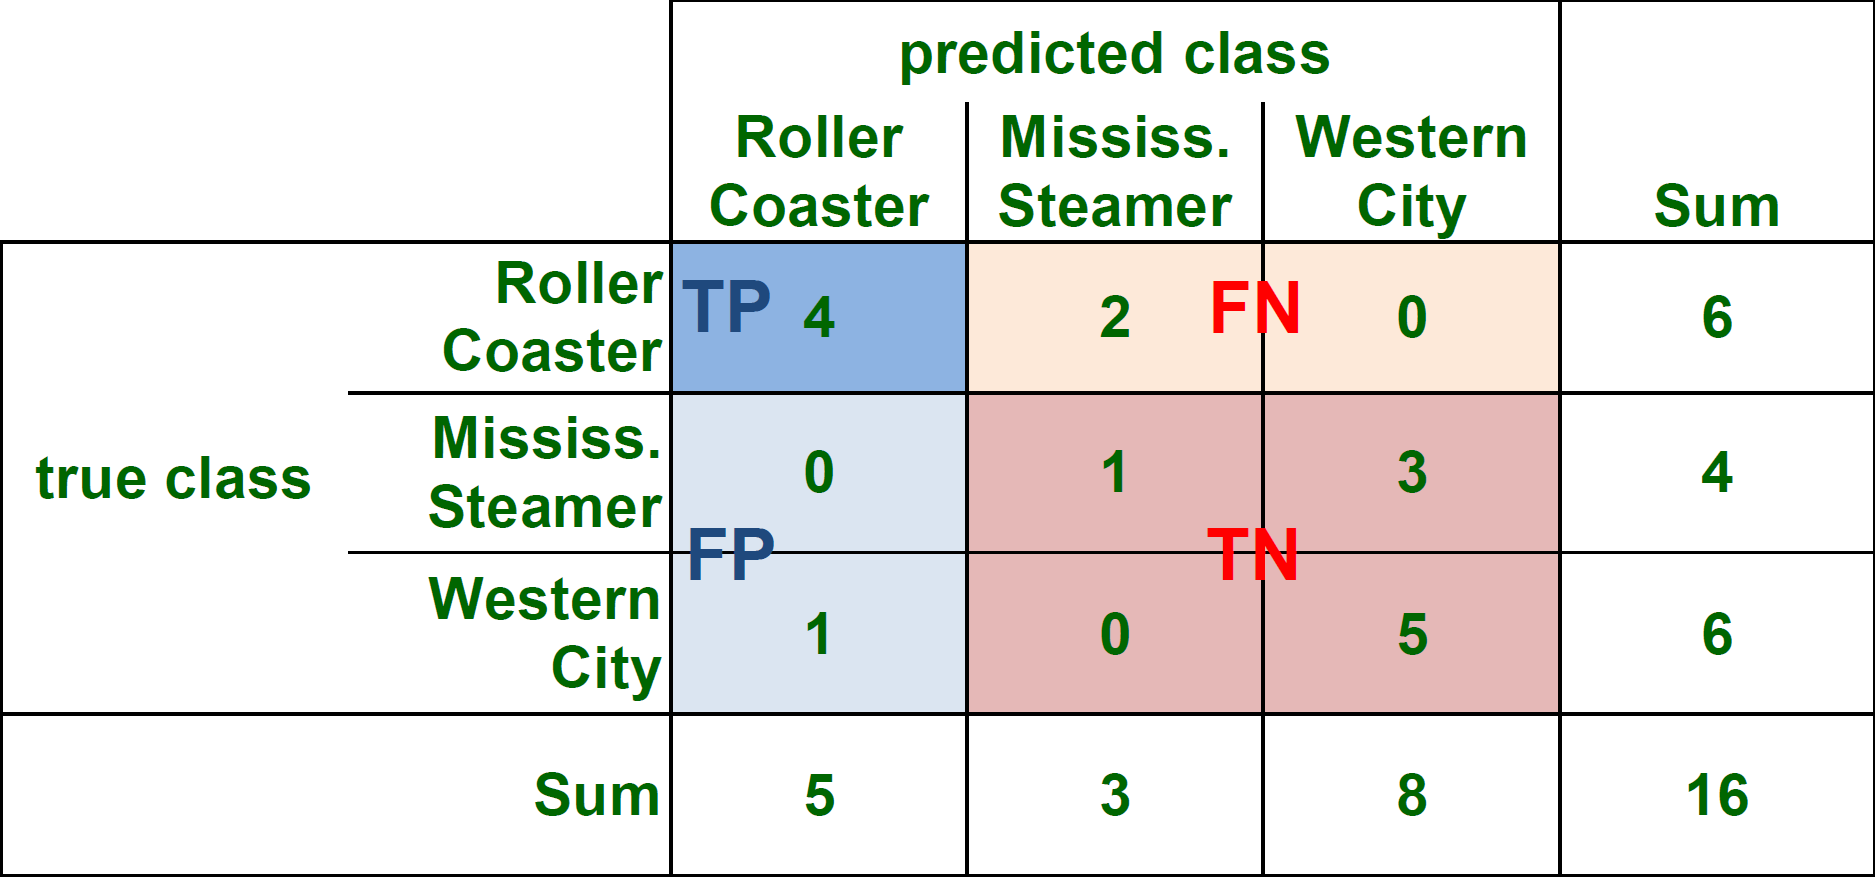
\includegraphics[width=.16\textwidth]{slides_images/confusion_matrix_theme_park}

Indicators:

\begin{itemize}
	\item True positives:
	\begin{itemize}
		\item target class, predicted correctly
		\item instances classified as ''RC'' \textbf{being indeed ''RC'': $2+2=4$}
	\end{itemize}
	\item False positives:
		\begin{itemize}
			\item target class predicted, actual class is different
			\item instances classified as ''RC'' but \textbf{being of some other class: $1$}		
		\end{itemize}
	\item True negatives:
		\begin{itemize}
			\item instances classified as not ''RC'' and \textbf{being indeed not ''RC'': $3 + 5 + 1 = 9$}
			\item contrast class, predicted correctly
		\end{itemize}
	\item False negatives: 
		\begin{itemize}
			\item constract class predicted, actual class different
			\item instances classified as not ''RC'' but \textbf{''RC'' though: $2$}
		\end{itemize}
	\item Precision = TP/(TP+FP) = $4/(4+1)=0.8$
	\item Recall = TP/(TP+FN) = $4/(4+2)=0.67$
\end{itemize}



\end{breakbox}

